\documentclass[12pt,a4paper]{article}
\usepackage{amsmath}
\usepackage{mathrsfs}
\usepackage{color}
\usepackage{tikz}
\usepackage{url}
%
\title{Inversion based on simultaneous observations of voltage and calcium concentration in iPSC-CMs}
\author{Joanneke E. Jansen}
%
\begin{document}
%
\maketitle
%
\section{Introduction} \label{Introduction}
In this report, we will investigate an inverse problem based on simultaneous observations of voltage and intracellular calcium concentration. Mathematically, inversion means the computation of the most plausible values of not directly observable parameters using a set of measurements. The classic technique to estimate electro-physiological cardiac parameters is patch clamping. With patch clamping, the transmembrane voltage of a single cell can be precisely measured over time. An alternative for the time and labour intensive patch clamping technique could be optical mapping, with which voltage and calcium waves of a cluster of cells can be measured simultaneously \cite{Lee2012}. The monodomain model is a commonly used model to simulate cardiac electro-physiology. Here, we will look if we can use this monodomain model to infer parameters based on voltage and intracellular calcium measurements, breaking the single cell tradition. As a motivating example, we will model the behaviour of monolayers of human incuduced pluripotent stem cell-derived cardiomyocytes (iPSC-CMs). In recent years, there has been a large interest in iPSC-CMs as a tool for drug screening and disease modelling and more efficient techniques for doing so are needed.
%
\subsection{Human induced pluripotent stem cell-derived cardiomyocytes (iPSC-CMs)}
Human induced pluripotent stem cell-derived cardiomyocytes (iPSC-CMs) provide a promising platform for studying cardiac cells in vitro. In 2007, it was first described how iPSCs can be made by reprogramming somatic cells \cite{Takahashi2007}. Since then, there has been a large interest in using those cells for drug safety screening and disease modelling \cite{Sallam2016}. Human iPSCs are self-renewing, patient-specific, and can be differentiated to cell types such as cardiomyocytes, hepatocytes and neurons \cite{Rajamohan2013}. In recent years, the techniques for efficiently producing homogeneous populations of iPSC-CMs  have greatly improved. However, the production process of iPSC-CMs is still very expensive in comparison to most \textit{in vitro} models. The largest limitation of the currently produced iPSC-CMs is their immature, and heterogeneous phenotype: the grown iPSC-CMs are typically a mix of ventricular-, atrial-, and nodal-like cells, although improvements in maturity and homogeneity are still being made \cite{Denning2016}. 
%
\subsection{Optical mapping}
There are several techniques to study the electrophysiology of iPSC-CMs. The method most commonly used is patch clamping. With this technique the transmembrane potential $v$ of a single cell can be precisely measured, but patch clamping is time and labour intensive, and thus precludes efficient large-scale screening. An alternative to patch clamping is optical mapping, using voltage-sensitive dyes (VSDs) or genetically-encoded voltage indicators (GEVIs) \cite{Denning2016}. With optical mapping, the transmembrane potential $v$ can be measured with a high spatial and temporal resolution. Unlike the invasive patch clamping technique, optical mapping allows for action potential measurements of large cell populations and sequential measurements of the same groups of cells for a longer period of time. Furthermore, it is possible to not only measure the transmembrane potential, but also the intracellular calcium concentration $[Ca]_i$, simultaneously \cite{Lee2012}. 
Although optical mapping methods do not produce action potential measurements that are equivalent to the golden standard patch clamp measurements, recent proof of principle studies have shown that they might be similar enough to be used for disease modelling and drug testing \cite{Shukla2017}. In \cite{Dempsey2016}, for example, simultaneous measurements of voltage and calcium with the genetically encoded calcium and voltage reporter CaViar was used for to screen the cardiotoxicity of drugs. Further, in \cite{Chen2016},
a cardiac subtype specific GEVI was used, thus allowing for subtype specific screening. However, those studies do not take in account the spatial resolution that optical mapping allows for. We will investigate what extra information those multiple cell measurements, such as the $\ge1$ cm large- diameter iPSC-CMs monolayer simultaneous voltage and calcium recordings from \cite{Lee2012}, can give us.
%
\subsection{Overview}
The aim of this report is to investigate the possibilities of parameter estimation of iPSC-CMs based on data obtained by optical mapping. In particular, we are interested to see what extra information can be inferred from the high spatial resolution and simultaneous calcium and voltage recordings, in contrast to the single cell voltage recordings obtained by patch clamping. We will model the behaviour of a monolayer of iPSC-CMs with the classic monodomain equations, which we will introduce in Section \ref{The monodomain model}. To model the cell membrane dynamics, we will use the Paci2013 cell model. The Paci2013 cell model is specifically developed for the simulation of iPSC-CMs action potentials and is based on data obtained on iPSC-CMs \cite{Paci2013, Ma2011}. Due to the already mentioned immature phenotype of currently produced iPSC-CMs, there is a lot of variability in the action potential shape of different cells, even if they are part of the same cell cluster \cite{Blazeski, Zhu2016}. Therefore, the predictive value of the Paci2013 and other cell models will be limited and our investigation must be seen as a proof of concept. The development of iPSC-CMs technologies is rapid and it is hoped that future iPSC-CMs will be more homogeneous and similar to mature cardiomyocytes\cite{Denning2016}. 
%
\section{Mathematical models} \label{Mathematical models}
\subsection{The monodomain model} \label{The monodomain model}
The monodomain equations are given by 
\begin{eqnarray} \label{eq:a}
\frac{\partial \mathbf{s}}{\partial t}= \mathbf{F}(\mathbf{s},v), \qquad \mathbf{x} \in H, \\
\frac{\partial v}{\partial t} + I_{ion}(v,\mathbf{s}) =\nabla \label{eq:b} \cdot(\mathbf{M}\nabla v) + I_s,\qquad \mathbf{x} \in H, \\ \label{eq:c}
\mathbf{n}\cdot (\mathbf{M}\nabla v)=0, \qquad \mathbf{x} \in \delta H,
\end{eqnarray}
with $v(\mathbf{x},t)$ the transmembrane potential (in mV), $H$ the domain, $\delta H$ the boundary of $H$, $\mathbf{n}$ the outward pointing normal of the boundary, and with $I_s$ the prescribed input current (in mV/ms) and $I_{ion}$ the ionic current across the membrane (in mV/ms), both scaled by the cell membrane capacitance (in $\mu$F/(mm$^2$)). 
Equation \eqref{eq:a} is a system of ODE's that models the membrane dynamics. There exist many different cell membrane dynamics models with varying degrees of complexity that can be used to specify $I_{ion}$, $\mathbf{F}(\mathbf{s},v)$ and the state variables $\mathbf{s}$, see the CellML repository \cite{cellml} for an overview of different types of models. In this report, we will use the Paci2013 cell model, that is specifically developed to model the electrophysical behaviour of iPSC-CMs \cite{Paci2013}. We will introduce the Paci2013 cell model in the next section.\\ Finally, $\mathbf{M}$ is a conductivity tensor (in mm$^2$/ms), that satisfies 
\begin{equation}
\mathbf{M}=\frac{\alpha}{1+\alpha}\mathbf{M}_i,\label{eq:d}
\end{equation}
with $\mathbf{M}_e=\alpha \mathbf{M}_i$. Here, $\mathbf{M}_e$ and $\mathbf{M}_i$ are the extracellular and intracellular conductivities (in mm$^2$/ms), divided by the product of the membrane capacitance (in $\mu$F/(mm$^2$)) and the cell membrane area-to-volume ratio (in 1/mm). By assuming that there exists a $\alpha$ such that $\mathbf{M}_e=\alpha \mathbf{M}_i$ the monodomain equations can be derived from the more complicated bidomain equations \cite[p. 566-568]{KeenerII}.
%
\subsection{The Paci2013 cell model} \label{The Paci2013 cell model}
The Paci2013 model consists of 18 ODEs and is of Hodgkin-Huxley type (see \cite[p. 195-215]{KeenerI} for an introduction to the Hodgkin-Huxley equations). The ionic current $I_{ion}$ is a sum of twelve different ion channel type currents:
\begin{eqnarray}
I_{ion}=I_{Na}+I_{CaL}+I_f+I_{K1}+I_{Kr}+I_{Ks}+ \\
I_{to}+I_{NaCa}+I_{NaK}+I_{pCa}+I_{bNa}+I_{bCa}.
\end{eqnarray}
An ion channel current $I_k$ is typically of the form 
\begin{equation}
I_{k}=g_k m_k^{p_k}\ldots h_k^{q_k}(u_m-u_k),
\end{equation}
where $g_k$ is the maximum conductance $g_k$ (in $\mu$S/$\mu$m$^2$), $u_k$ (in mV) the Nernst potential and $m_k$, $h_k \ldots$ are a certain number of voltage and time dependent gating variables. Each ion channel type has different types and/or numbers of gating variables. The Paci2013 model contains ODEs to describe the dynamics of thirteen different ionic gating variable types. Apart from the ionic gating variables and an inner calcium dynamics gating variable, the state variables of the Paci2013 model also include the intracellular sodium and calcium, and the sarcoplasmic reticulum calcium concentrations $[Na]_i, [Ca]_i$ and $[Ca]_{SR}$ \cite{Paci2013}. The estimation of the model parameters is mainly based on patch clamp iPSC-CM data from \cite{Ma2011}. The iPCS-CMs studied by \cite{Ma2011} showed atrial-, nodal-, and ventricular-like action potentials. The Paci2013 model contains of two sets of parameters: one to simulate ventricular-like cells and one to simulate atrial-like cells. We will call those two models the ventricular and atrial Paci2013 model respectively.
%
\section{Basic test case} \label{Basic test case}
For our test case, we take a rectangular strip of $12$ mm $\times\: 0.01$ mm as our domain. We solve our test case with the \url{splittingsolver} module (first order Godunov splitting scheme) from the cbcbeat Python package. \cite{cbcbeat}\footnote{This electrophysiology solver package is based on the FEniCS Project software \cite{fenics} and the dolfin-adjoint software \cite{dolfin-adjoint}. We use a first order Godunov splitting scheme, a 1st order Rush-Larsen scheme for the ODEs and the CG algorithm with PETSc AMG preconditioner.} The \url{splittingsolver} solves the monodomain PDE system and its coupled cell membrame dynamics ODE system separately, using the operator splitting scheme as described in \cite{Sundnes}. We retrieved the code for the Paci2013 cell models from the CellML repository: \url{http://models.cellml.org/e/16d/}. With a few minor adjustments\footnote{i.e. adding of necessary parentheses, fixing integer division, renaming of the membrane potential, removing the inbuilt stimulus and adding of the after conversion mysteriously dissapeared part of the \url{m_inf} parameter.}, we could convert the models to cbcbeat versions.  We take typical values $\sigma_l=0.15$ and $\sigma_t=0.02$ (in mS/mm) for the longitudinal and tangential conductivity respectively and take $C_m=0.2$ for the membrane capacitance (in $\mu$F/(mm$^2$)) and $\beta=200$ for the cell membrane area-to-volume ratio (in 1/mm) \cite{Roth}, data from \cite{Plonsey1882, Plonsey1984}. Without a stimulus, both the atrial and ventricular Paci2013 models beat spontaneously. We did not investigate this spontaneously beating, but applied a 1 Hz stimulus instead, as we assumed that this would produce more useful measurements in practice. Further, we only investigated the ventricular model. We choose the ventricular model because ventricular cells are more common than atrial cells and also the ones mainly used for drug tests \cite{Paci2015}.
We ran the model for 800 s to reach a steady state, while applying a $1$ Hz stimulus of $5$ ms and $5.6$ A/F, the default stimulus values of the Paci2013 ventricular model, over the left $25\%$ of the domain, and then recorded the membrane potential and intracellular calcium concentration for $2$ s. In Figure \ref{fig:1}, we show a heat map of $v$ at $t=5, 15, 40$ and $80$ ms after we started our recordings. A stimulus was applied during the first $5$ ms over the left $25\%$ of the domain. In Figure \ref{fig:2}, we show a heat map of $[Ca]_i$ at the same times. In Figure \ref{fig:3}, we plot $v$ and $[Ca]_i$ over time, both at a point at the left of the domain (in blue, at ($5$ mm, $0$ mm)) and at a point at the right of the domain (in red, at ($10$ mm, $0$ mm)).
%
\begin{figure}
\begin{minipage}{0.47\textwidth}
 \textbf{(a)} 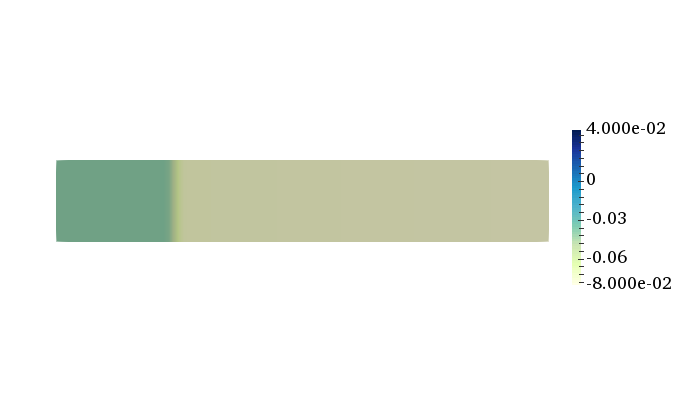
\includegraphics[trim=9cm 0cm 2cm 0cm, clip=true, width=0.9\linewidth]{v5}
      \textbf{(c)} 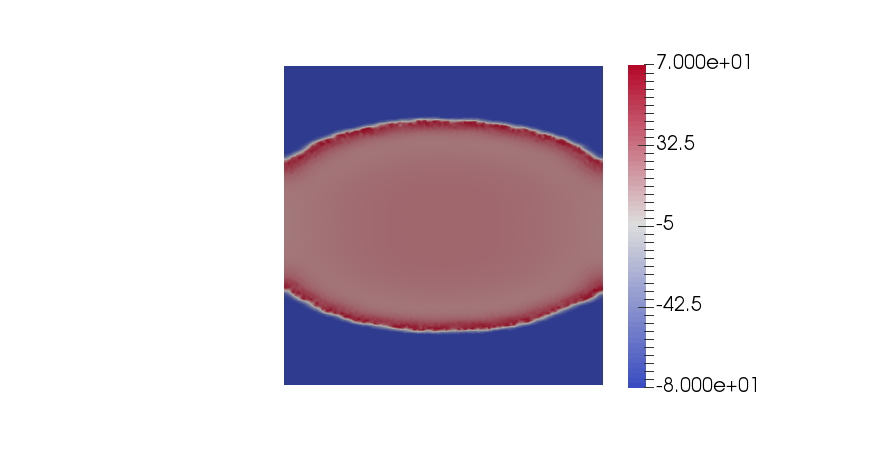
\includegraphics[trim=9cm 0cm 2cm 0cm, clip=true, width=0.9\linewidth]{v40}
    \end{minipage}
    \begin{minipage}{0.47\textwidth}
  \textbf{(b)} 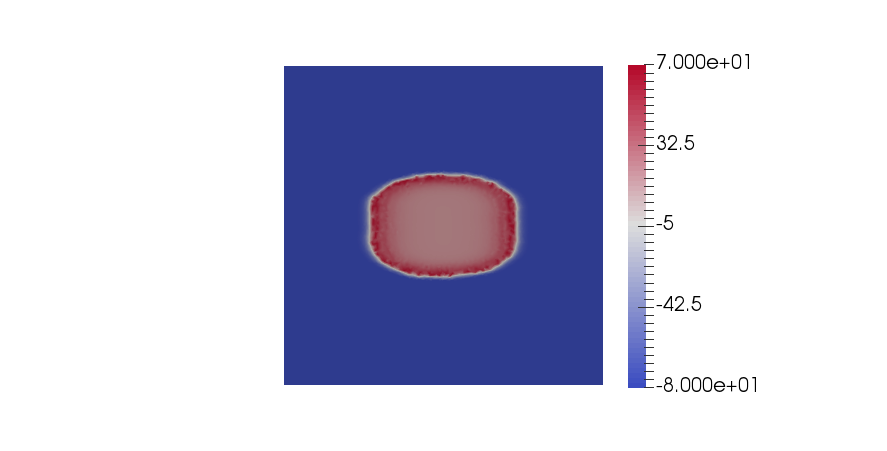
\includegraphics[trim=9cm 0cm 2cm 0cm, clip=true, width=0.9\linewidth]{v15}
  \textbf{(d)} 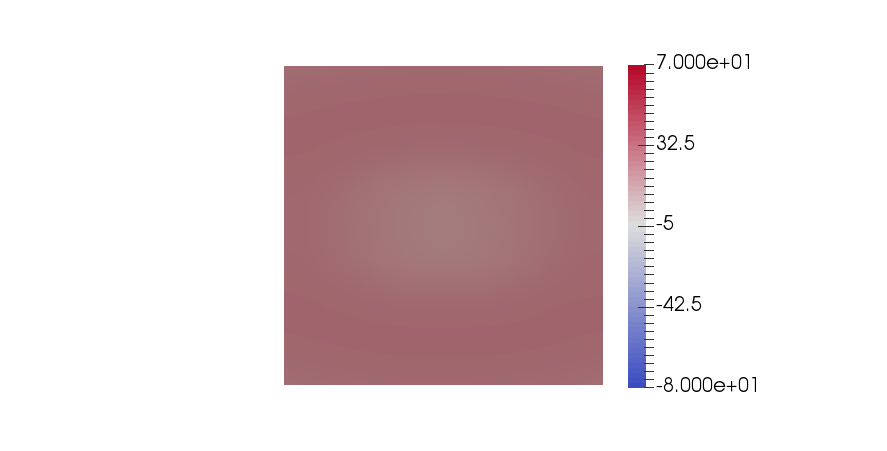
\includegraphics[trim=9cm 0cm 2cm 0cm, clip=true, width=0.9\linewidth]{v90}
    \end{minipage}
    \caption{Heat maps of $v$ (in mV) of our basic test case at \textbf{(a)} $t=5$ms, \textbf{(b)} $t=15$ms, \textbf{(c)} $t=40$ms and \textbf{(d)} $t=80$ms.}
    \label{fig:1}
\end{figure}
%
\begin{figure}
\begin{minipage}{0.47\textwidth}
 \textbf{(a)} 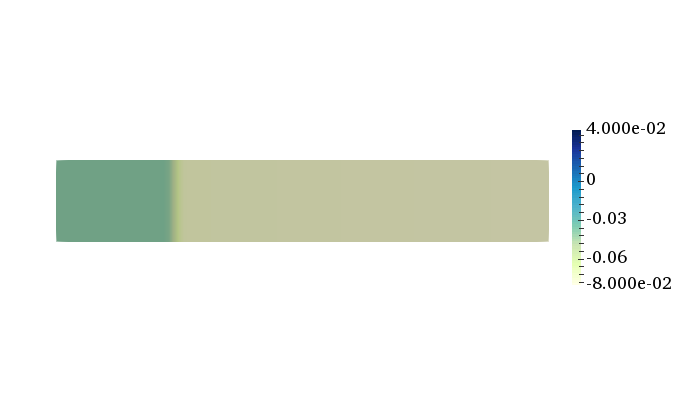
\includegraphics[trim=9cm 0cm 2cm 0cm, clip=true, width=0.9\linewidth]{v5}
      \textbf{(c)} 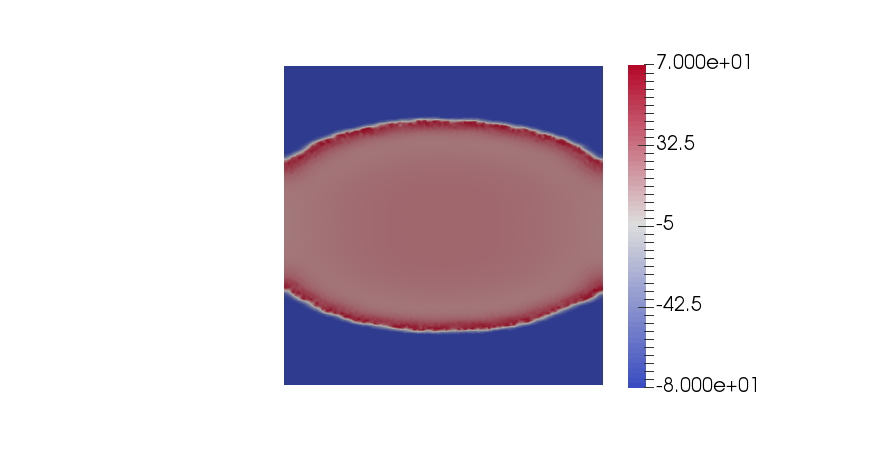
\includegraphics[trim=9cm 0cm 2cm 0cm, clip=true, width=0.9\linewidth]{v40}
    \end{minipage}
    \begin{minipage}{0.47\textwidth}
  \textbf{(b)} 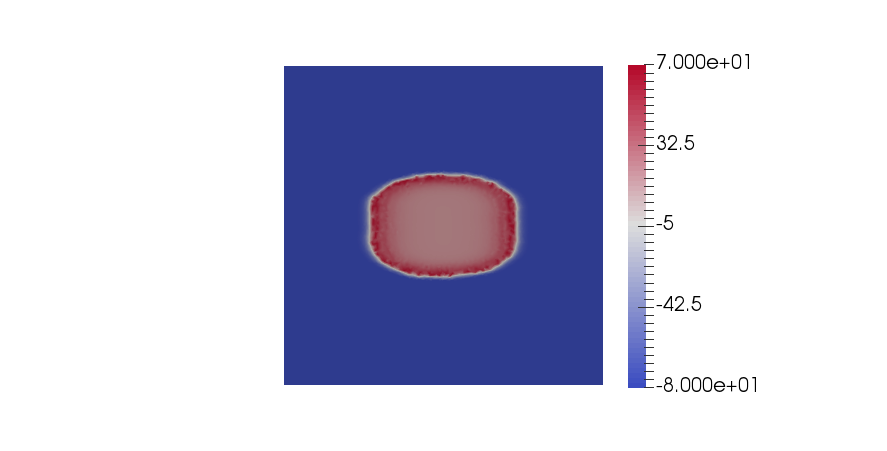
\includegraphics[trim=9cm 0cm 2cm 0cm, clip=true, width=0.9\linewidth]{v15}
  \textbf{(d)} 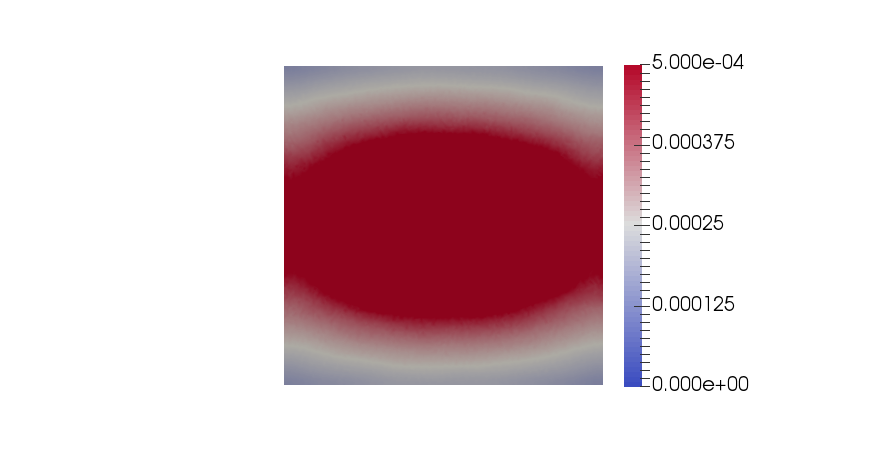
\includegraphics[trim=9cm 0cm 2cm 0cm, clip=true, width=0.9\linewidth]{Casl80}
    \end{minipage}
    \caption{Heat maps of $[Ca]_i$ (in $\mu$M) of our basic test case at \textbf{(a)} $t=5$ms, \textbf{(b)} $t=15$ms, \textbf{(c)} $t=40$ms and \textbf{(d)} $t=80$ms.}
    \label{fig:2}
\end{figure}
%trim={<left> <lower> <right> <upper>}
%
\begin{figure}
   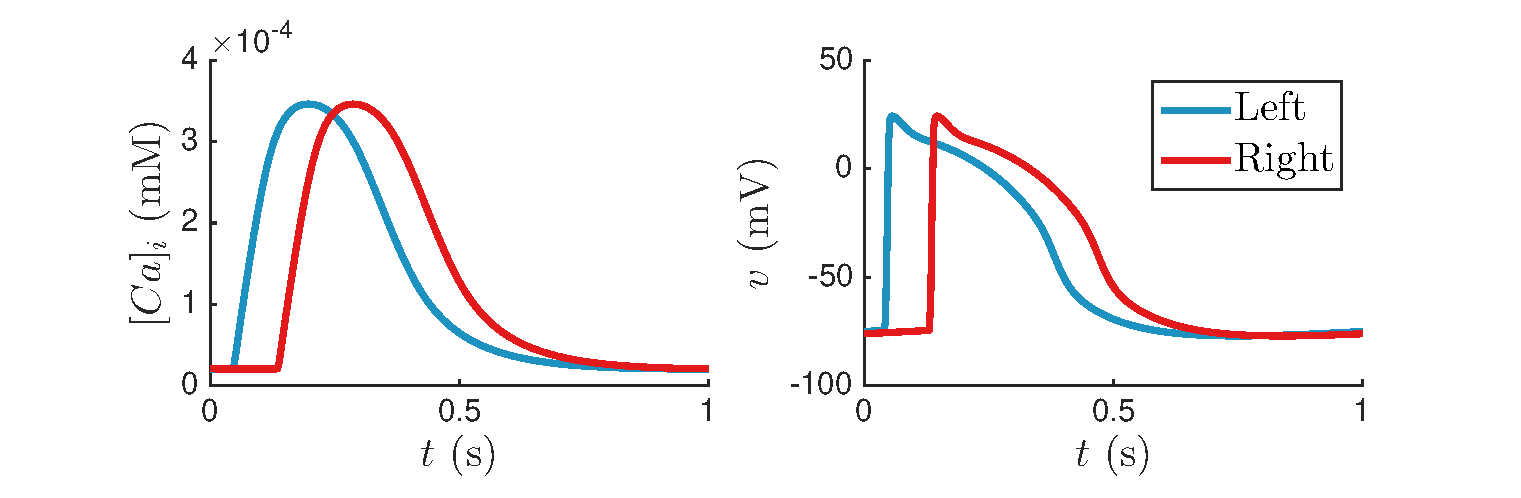
\includegraphics[width=1\linewidth]{strip} 
    \caption{Plot of $v$ and $[Ca]_i$ against $t$, at the left of the domain (in blue, at ($5$ mm, $0$ mm)) and at the right of the domain (in red, at at ($10$ mm, $0$ mm)) The total domain size is $12$ mm by $0.01$ mm.}
    \label{fig:3}
\end{figure}
%
\section{The inverse problem} \label{The inverse problem}
%It is possible to obtain measurements $u_{\text{obs}}$ of the transmembrane potential and measurements $c_{\text{obs}}$ of the cytosolic calcium concentration $[Ca]_i$ over the whole domain $H$ at discrete points in time. With those measurements, we can estimate the value of the parameters in our model, using an adjoint-based approach.\footnote{See, for example, \cite{Gunzburger} for an introductory text in adjoint-based optimization methods.} Here, as an example, we will try to estimate the values of the $\sigma_l$ parameter from the Grandi cell model.
%We can formulate this problem as an optimisation problem: find $\sigma_l$, such that the functional
%\begin{eqnarray}
%\mathcal{J}(v, [Ca]_i, \sigma_l)= \frac{1}{N} \sum_{i=1}^{N} \frac{||v-v_{\text{obs}}(t_i)||^2_{L^2}}{||v_{\text{obs}}(t_i)||^2_{L^2}} + \frac{||[Ca]_i-[Ca]_{i\text{obs}}(t_i) ||^2_{L^2}}{||[Ca]_{i\text{obs}}(t_i) ||^2_{L^2}},\label{J}
%\end{eqnarray}
%%\begin{eqnarray} \nonumber
%%\mathcal{J}(v, c, \sigma_l)= \\ \frac{1}{N} \sum_{i=1}^{N} \int_{H}(v(\textbf{x},t_i)-\Phi(\textbf{x},t_i))^2 \: \text{d}\textbf{x} + \int_{H}\left(c(\textbf{x},t_i)-\Psi(\textbf{x},t_i)\right)^2 \: \text{d}\textbf{x},\label{J}
%%\end{eqnarray}
%is minimized, subject to the requirements that $v, c$ and $\sigma_l$ satisfy the state system of equations \eqref{eq:a}-\eqref{eq:c} and initial conditions $v(\textbf{x},0)=v_0(\textbf{x})$ and $\mathbf{s}(\mathbf{x},0)=\mathbf{s}_0(\mathbf{x})$. Here, $N$ are the number of measurements in time and $t_i$, $i=1, \dots N$ the respective moments in time.
%% https://fenicsproject.org/qa/6675/hdf-file-read-write-for-time-series
%Using cbcbeat and the dolfin-adjoint software on which it is based, we can automatically compute the total derivative of $\mathcal{J}$ with respect to the optimization parameter $\sigma_l$. We can then use the scipy optimisation algorithm \url{minimize()} -which uses the limited memory Broyden–Fletcher–Goldfarb–Shanno (BFGS) method with bound support - to find an optimal value for $\sigma_l$. We first generated some fake observed data for $\sigma_l=0.15$, from $t=0.0$ to $t=5.0$ ms, with a timestep $dt=0.05$ ms. With $\sigma_l=0.10$ as initial guess, the \url{minimize()} algorithm returned $\sigma_l=?$ after ? iterations. Similarly, we can optimize for other parameters, such as $\sigma_t$, or $g\_Na$, $g\_CaL$, $g\_K1$ or $g\_K2$ from the Grandi cell model. 
%
%%With $\sigma_t=0.01$ as initial guess and fake data created for $\sigma_t=0.02$, the \url{minimize()} algorithm converged to $\sigma_t=0.020005$ after five iterations. Optimizing for both $\sigma_l$ and $\sigma_t$, with the same initial guesses and synthetic data, gave convergence in eight iterations. The value of the functional at each iteration step was consecutively $38.6, 11.7, 10.0, 3.19, 0.89, 0.023, 0.00063, 0.0000084$ and $0.0000098$. We also looked at synthetic spatially varying $\sigma_l$ and $\sigma_t$$\ldots$
%
\section{Conslusion} \label{Conclusion}
%
\begin{thebibliography}{99}
\bibitem{Blazeski} Blazeski, A., Zhu, R., Hunter, D. W., Weinberg, S. H., Boheler, K. R., Zambidis, E. T., \& Tung, L. (2012). Electrophysiological and contractile function of cardiomyocytes derived from human embryonic stem cells. \textit{Progress in Biophysics and Molecular Biology, 110}(0), 178–195.
\bibitem{Chen2016} Chen, Z., Xian, W., Bellin, M., Dorn, T., Tian, Q., Goedel, A., \ldots Hinkel, R. (2016). Subtype-specific promoter-driven action potential imaging for precise disease modelling and drug testing in hiPSC-derived cardiomyocytes. \textit{European Heart Journal, 38}, 292-301.
\bibitem{Dempsey2016} Dempsey, G. T., Chaudhary, K. W., Atwater, N., Nguyen, C., Brown, B. S., McNeish, J. D., \ldots Kralj, J. M. (2016). Cardiotoxicity screening with simultaneous optogenetic pacing, voltage imaging and calcium imaging. \textit{Journal of pharmacological and toxicological methods, 81}, 240-250.
\bibitem{Denning2016} Denning, C., Borgdorff, V., Crutchley, J., Firth, K. S., George, V., Kalra, S., \ldots Prodanov, L. (2016). Cardiomyocytes from human pluripotent stem cells: from laboratory curiosity to industrial biomedical platform. \textit{Biochimica et Biophysica Acta (BBA)-Molecular Cell Research, 1863}(7), 1728-1748.
\bibitem{Lee2012} Lee, P., Klos, M., Bollensdorff, C., Hou, L., Ewart, P., Kamp, T. J., \ldots Jalife, J. (2012). Simultaneous Voltage and Calcium Mapping of Genetically Purified Human Induced Pluripotent Stem Cell–Derived Cardiac Myocyte MonolayersNovelty and Significance. \textit{Circulation research, 110}(12), 1556-1563.
\bibitem{Leyton2014} Leyton-Mange, J. S., Mills, R. W., Macri, V. S., Jang, M. Y., Butte, F. N., Ellinor, P. T., \& Milan, D. J. (2014). Rapid cellular phenotyping of human pluripotent stem cell-derived cardiomyocytes using a genetically encoded fluorescent voltage sensor. \textit{Stem Cell Reports, 2}(2), 163-170.
\bibitem{Ma2011} Ma, J., Guo, L., Fiene, S., Anson, B., Thomson, J., Kamp, T., \ldots January, C. (2011). High purity human-induced pluripotent stem cell-derived cardiomyocytes: Electrophysiological properties of action potentials and ionic currents. \textit{American Journal of Physiology. Heart and Circulatory Physiology, 301}(5), H2006-17.
\bibitem{KeenerI} Keener, J. P., \& Sneyd, J. (2009). \textit{Mathematical physiology (Vol. I)}. New York: Springer.
\bibitem{KeenerII} Keener, J. P., \& Sneyd, J. (2009). \textit{Mathematical physiology (Vol. II)}. New York: Springer.
\bibitem{Paci2013} Paci, M., Hyttinen, J., Aalto-Set\"al\"a, K., \& Severi, S. (2013). Computational models of ventricular-and atrial-like human induced pluripotent stem cell derived cardiomyocytes. \textit{Annals of biomedical engineering, 41}(11), 2334-2348.
\bibitem{Paci2015} Paci, M., Hyttinen, J., Rodriguez, B., \& Severi, S. (2015). Human induced pluripotent stem cell‐derived versus adult cardiomyocytes: An in silico electrophysiological study on effects of ionic current block. \textit{British Journal of Pharmacology, 172}(21), 5147-5160.
\bibitem{Plonsey1882} Plonsey, R., \& Barr, R. (1982). The Four-Electrode Resistivity Technique as Applied to Cardiac Muscle. \textit{Biomedical Engineering, IEEE Transactions on, BME-29}(7), 541-546.
\bibitem{Plonsey1984} Barr, \& Plonsey. (1984). Propagation of excitation in idealized anisotropic two-dimensional tissue. \textit{Biophysical Journal, 45}(6), 1191-1202.
\bibitem{Rajamohan2013} Rajamohan, D., Matsa, E., Kalra, S., Crutchley, J., Patel, A., George, V., \& Denning, C. (2013). Current status of drug screening and disease modelling in human pluripotent stem cells. \textit{Bioessays, 35}(3), 281-298.
\bibitem{Sallam2016} Sala, L., Bellin, M., \& Mummery, C. (2016). Integrating cardiomyocytes from human pluripotent stem cells in safety pharmacology: Has the time come?: Implementation of hiPSC-CMs in cardiotoxicity. \textit{British Journal of Pharmacology}.
\bibitem{Roth} Sepulveda, Roth, \& Wikswo. (1989). Current injection into a two-dimensional anisotropic bidomain. \textit{Biophysical Journal, 55}(5), 987-999.
\bibitem{Shukla2017} Shukla, P., \& Wu, J. (2016). Cardiac subtype characterization using all-optical action potential imaging. \textit{European Heart Journal, 38}(4), 302-304.
\bibitem{Sundnes} Sundnes, J., Nielsen, B., Mardal, K., Cai, X., Lines, G., \& Tveito, A. (2006). On the Computational Complexity of the Bidomain and the Monodomain Models of Electrophysiology. \textit{Annals of Biomedical Engineering, 34}(7), 1088-1097.
\bibitem{Takahashi2007} Takahashi, K., Tanabe, K., Ohnuki, M., Narita, M., Ichisaka, T., Tomoda, K., \& Yamanaka, S. (2007). Induction of pluripotent stem cells from adult human fibroblasts by defined factors. \textit{cell, 131}(5), 861-872.
\bibitem{Zhu2016} Zhu, R., Millrod, M. A., Zambidis, E. T., \& Tung, L. (2016). Variability of action potentials within and among cardiac cell clusters derived from human embryonic stem cells. \textit{Scientific reports, 6}, 18544.
\bibitem{cellml} \url{models.cellml.org/electrophysiology}
\bibitem{fenics} \url{fenicsproject.org}
\bibitem{dolfin-adjoint} \url{www.dolfin-adjoint.org}
\bibitem{cbcbeat} \url{bitbucket.org/meg/cbcbeat}
\end{thebibliography}
%
\end{document}